%%%%%%%%%%%%%%%%%%%%%%%%%%%%%%%%%%%%%%%%%
% Journal Article
% LaTeX Template
% Version 1.4 (15/5/16)
%
% This template has been downloaded from:
% http://www.LaTeXTemplates.com
%
% Original author:
% Frits Wenneker (http://www.howtotex.com) with extensive modifications by
% Vel (vel@LaTeXTemplates.com)
%
% License:
% CC BY-NC-SA 3.0 (http://creativecommons.org/licenses/by-nc-sa/3.0/)
%
%%%%%%%%%%%%%%%%%%%%%%%%%%%%%%%%%%%%%%%%%

%----------------------------------------------------------------------------------------
%	PACKAGES AND OTHER DOCUMENT CONFIGURATIONS
%----------------------------------------------------------------------------------------

\documentclass[twoside,twocolumn]{article}

\usepackage{blindtext} % Package to generate dummy text throughout this template 

\usepackage[sc]{mathpazo} % Use the Palatino font
\usepackage[T1]{fontenc} % Use 8-bit encoding that has 256 glyphs
\linespread{1.05} % Line spacing - Palatino needs more space between lines
\usepackage{microtype} % Slightly tweak font spacing for aesthetics

\usepackage[english]{babel} % Language hyphenation and typographical rules

\usepackage{graphicx}
\usepackage{amsmath}
\usepackage{txfonts}
\usepackage{tabularx}
\usepackage{listings}
\usepackage{float}
\usepackage{pbox}
\usepackage{color}
\usepackage{todonotes}

\usepackage[hmarginratio=1:1,top=32mm,columnsep=20pt]{geometry} % Document margins
\usepackage[hang, small,labelfont=bf,up,textfont=it,up]{caption} % Custom captions under/above floats in tables or figures
\usepackage{booktabs} % Horizontal rules in tables

\usepackage{lettrine} % The lettrine is the first enlarged letter at the beginning of the text

\usepackage{enumitem} % Customized lists
\setlist[itemize]{noitemsep} % Make itemize lists more compact

\usepackage{abstract} % Allows abstract customization
\renewcommand{\abstractnamefont}{\normalfont\bfseries} % Set the "Abstract" text to bold
\renewcommand{\abstracttextfont}{\normalfont\small\itshape} % Set the abstract itself to small italic text

\usepackage{titlesec} % Allows customization of titles
\renewcommand\thesection{\Roman{section}} % Roman numerals for the sections
\renewcommand\thesubsection{\roman{subsection}} % roman numerals for subsections
\titleformat{\section}[block]{\large\scshape\centering}{\thesection.}{1em}{} % Change the look of the section titles
\titleformat{\subsection}[block]{\large}{\thesubsection.}{1em}{} % Change the look of the section titles

\usepackage{fancyhdr} % Headers and footers
\pagestyle{fancy} % All pages have headers and footers
\fancyhead{} % Blank out the default header
\fancyfoot{} % Blank out the default footer
\fancyhead[C]{To Hop or Not to Hop $\bullet$ May 2018 $\bullet$ Vol. I, No. 1} % Custom header text
\fancyfoot[RO,LE]{\thepage} % Custom footer text

\usepackage{titling} % Customizing the title section
\usepackage{hyperref} % For hyperlinks in the PDF

\lstset{ %
	language=C,                % choose the language of the code
	basicstyle=\footnotesize,       % the size of the fonts that are used for the code
	numbers=none,                   % where to put the line-numbers
	numberstyle=\footnotesize,      % the size of the fonts that are used for the line-numbers
	stepnumber=1,                   % the step between two line-numbers. If it is 1 each line will be numbered
	backgroundcolor=\color{white},  % choose the background color. You must add \usepackage{color}
	showspaces=false,               % show spaces adding particular underscores
	showstringspaces=false,         % underline spaces within strings
	showtabs=false,                 % show tabs within strings adding particular underscores
	frame=single,           % adds a frame around the code
	tabsize=2,          % sets default tabsize to 2 spaces
	captionpos=b,           % sets the caption-position to bottom
	breaklines=true,        % sets automatic line breaking
	breakatwhitespace=false,    % sets if automatic breaks should only happen at whitespace
	escapeinside={\%*}{*)}          % if you want to add a comment within your code
}

%----------------------------------------------------------------------------------------
%	TITLE SECTION
%----------------------------------------------------------------------------------------

\setlength{\droptitle}{-4\baselineskip}

\pretitle{\begin{center}\Huge\bfseries}
\posttitle{\end{center}}
\title{Wireless Sensor Networks \\ To Hop or Not to Hop} % Article title
\author{
\textsc{David Jensen} \\[1ex]
\normalsize Stud. M.Sc. CE, ASE, Aarhus University \\
\href{mailto:11229@post.au.dk}{11229@post.au.dk}
\and
\textsc{Henrik Bagger Jensen} \\[1ex]
\normalsize Stud. M.Sc. CE, ASE, Aarhus University \\
\normalsize \href{mailto:201304157@post.au.dk}{201304157@post.au.dk}
\and
\textsc{Christian M. Lillelund} \\[1ex]
\normalsize Stud. M.Sc. CE, ASE, Aarhus University \\
\normalsize \href{mailto:201408354@post.au.dk}{201408354@post.au.dk}
\and
\textsc{Troels Thomsen} \\[1ex]
\normalsize Stud. M.Sc. ET, ASE, Aarhus University \\
\normalsize \href{mailto:09641@post.au.dk}{09641@post.au.dk}
}
\date{\today} % Leave empty to omit a date
\renewcommand{\maketitlehookd}{%
\begin{abstract}
\noindent Whether to relay data packets or to send them directly between two computers in a wireless network setting is a frequently discussed topic in computer engineering. Typically, when a consumer node cannot reach a wireless router in a wireless local area network (WLAN), other fixed access points in place must relay the packets of the consumer. In a wireless sensor network (WSN), other concerns come into play, such as network dynamicity, battery levels and noise interfence, which must be considered before relaying packets. In this project
we build a relaying protocol based on signal strength and accumulated transmission errors (lost packets) and use it to investigate what factors it pays for a WSN to relay by: The event quality (how many times did we notice an event), energy consumption aiming to use the least amount of energy to extend lifetime, or conceivably a comprimise of both. Events in our case is the heart rate of a athlete runner running a oval-formed running track. We find that creating such a multivariate decision protocol is indeed possible and our results show XXX
but using signal strentgh values from the CC2420 radio can be unreliable and that a wireless sensor node should only relay packets when it is absolutely necessary to reach a destination in order to save energy.
%TODO: Add results here.
\end{abstract}
}

%----------------------------------------------------------------------------------------

\begin{document}

% Print the title
\maketitle

%----------------------------------------------------------------------------------------
%	ARTICLE CONTENTS
%----------------------------------------------------------------------------------------

\chapter{Introduction}\label{ch:introduction}

This report details a project done in Wireless Sensor Networks (WSN) with a mini-project called "To hop or to hop". The project follows the original idea of determining when to relay packets in a wireless network, but with a little twist to it - instead of placing the receiving node in a fixed position, we place it on an athlete running a marathon on a oval-formed running track in order to measure his heart rate every minute. This information is going to be transfered to a sink (base station) over a wireless connection with an added two relay stations in between that help ensure sufficient network coverage of the track. To design the track for our purpose, we will employ knowledge of fading, radio wave propagation and received input power (dbM) in a wireless node.

\noindent We will look to create an effective protocol that can determine when to communicate directly with the node based on the athlete and when it is best to use one of the relays. This protocol will take signal strength and energy consumption into consideration. For inter-node connectivity, we will design and implement the data-link layer stop-and-wait ARQ protocol on all nodes.

\noindent With reference to the mini-project presentation, we use telosb nodes all running TinyOS with a packet size of 128 bytes. The RF transceiver is a single-chip 2.4 GHz IEEE 802.15.4 compliant CC2420 with a data rate of 250 kbps.

\section{Scenario Introduction}\label{sc:scenarioIntroduction}
% Scenario introduction
A marathon runner is racing a track shaped as shown in figure 1, while equipped with sensor node A. The sensor node is broadcasting four packages per second tracking the runner’s pulse history. The level of details in the tracking package defines the number of marathons possible for the runner to run before a new battery is required. At one time the track was closed, resulting in the runner racing around the building of her workplace.

\begin{figure}[H]
	\centering
	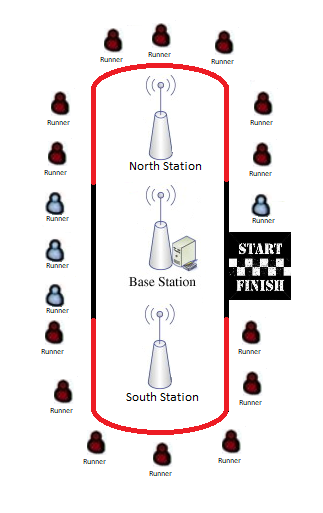
\includegraphics[width=\linewidth]{introduction/scenario/fig/scenarioIntroduction.png}
	\caption{A marathon runner "node A" is racing around a track, while transmitting pulse information to the base station. In the red northern territory, node A transmits to the north station which relays the message to the base station. Likewise, at the southern station.}
	\label{fig:scenarioIntroduction}
\end{figure}

\section{Protocol introduction “To hop or not to hop”}\label{sc:protocolIntroduction}
Node A will be broadcasting with a packet size of 128 Bytes. The base station will collect the data from node A when in range and save the data. The North station will, when in range and the base station is out of range, receive and relay the message to the base station. The same scenario will happen at the south station. Time Synchronization, Localization and Scalability will be considered regarding the protocol design. Each and combined scenarios will be evaluated in relation to signal strength relative to power consumption and data reliability. 

\chapter{Theory}\label{ch:theory}

This chapter will introduce theory concepts used in this project. We will cover both antenna theory, go into detail about fading and explain how the ARQ method works.

\section{Path Loss "Free Space Loss vs engineering building space loss"}\label{sc:pathLoss}
To be able to understand the need for relaying, one must first understand the boundaries of the chosen working environment. The range equation gives a nice theoretical reference point to how a far a certain quality signal can be transmitted in optimal conditions. The range equation is dependent on transmission frequency and characteristics of the transmitting and receiving antenna. The frequency dependency comes from the range equation calculation of the far field distance from the antenna pair. The far field distance is when the magnetic and electric part of the signal has a steady state phase relation. Also, the far field distance is dependent on the size and type of the antenna, while the Telosb has a 2.7cm inverted f-antenna and it is transmitting at $2.408GHz$ centre frequency. $2.408GHz$ transmission frequency is chosen from the standard IEEE\_802.15.4, making $2.401GHz$ a ‘1’ and $2.408$ a ‘0’. Trying to keep the frequency as low as possible gives longer transmit range both in theory and in practice, as the lower frequencies have better penetration chances given obstacles. The radiation pattern, $-3dB$ power line, of a Ferrite-based inverted F-antenna can be seen in Figure \ref{fig:invertedAntenna} [6]. Focusing on protocol and power consumption the range equation will be visualized based on an omnidirectional antennas with same polarization, isotropic.

\begin{figure}[H]
	\centering
	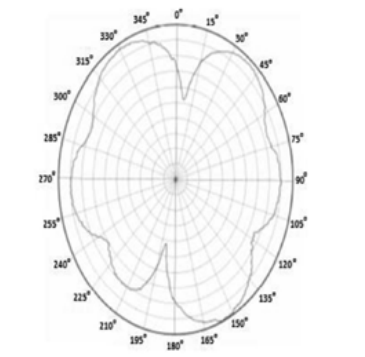
\includegraphics[width=0.8\linewidth]{theory/pathLoss/fig/invertedAntenna.png}
	\caption{Estimation of an inverted F-Antenna radiation pattern.}
	\label{fig:invertedAntenna}
\end{figure}

Telosb software specifies transmission power in dBm and the receiving and transmitting antenna have same characterises, so the need to understand the antenna characteristics beyond the far field distance estimation is not needed for this project. Since the main scope of the project is package control protocol, each antenna is treated as an isotropic antenna being able to broadcast up to $100m$ in each direction as specified in the datasheet. To simulate a real scenario the transmitting antenna could be mounted on a rotational motor following the runner through computer vision hence the main beam, e.g. $153\deg$, of the antenna pattern would always point towards the runner verifying our calculation approach. Giving a far field distance of $0.01167m$ and optimal conditions in air, Figure \ref{fig:logpathReceivedSignal_baseStation_air_highSignal} shows the expected received signal strength indication, RSSI, based on the range equation, Equation \ref{eq:rangeEquation} and presumed assumptions.



\begin{figure}[H]
	\begin{flalign*}
		f &= 2.407 \cdot 10^{9} Hz \qquad
		D = 2.7 \cdot 10^{-3} m \\
		\lambda &= \frac{c}{f} = 0.125m \qquad
		\gamma_{air} = 2 \qquad
		\gamma_{building} = 5.5\\
		d{0} &= \frac{2 \cdot D^{2}}{\lambda} = 1.171 \cdot 10^{-4} m
	\end{flalign*}
	
	\begin{subequations}
		\label{eq:rangeEquation}
		\begin{align}
			P_{rcvd}(d) &= \frac{ P_{tx} \cdot G_{t} \cdot G_{r} \cdot \lambda^{2} }{ (4 \pi)^{2} \cdot d^{2} \cdot L }\\
			&= \frac{ P_{tx} \cdot G_{t} \cdot G_{r} \cdot \lambda^{2} }{ (4 \pi)^{2} \cdot d_{0}^{2} \cdot L } \cdot \bigg (\frac{d_{0}}{d} \bigg )^{2}\\
			&= P_{rcvd}(d_{0}) \cdot \bigg (\frac{d_{0}}{d} \bigg )^{\gamma}
		\end{align}
	\end{subequations}
	\caption{Range equation based on a $2.7cm$ wide inverted f-antenna and a $2.408GHz$ center frequency}
\end{figure}

%Figure 3
\begin{figure}[H]
	\centering
	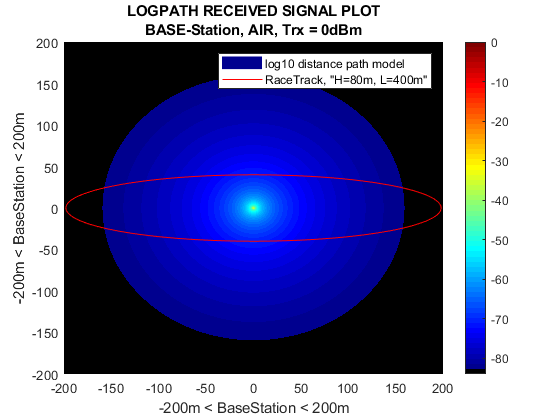
\includegraphics[width=\linewidth]{theory/pathLoss/fig/logpathReceivedSignal_baseStation_air_highSignal.png}
	\caption{$-84dBm$ $159.3m$ received signal area of the race track. The antenna cannot cover the entirety of the racetrack.}
	\label{fig:logpathReceivedSignal_baseStation_air_highSignal}
\end{figure}


Given a racetrack of $400m$ in width, under optimal conditions, as shown in Figure \ref{fig:logpathReceivedSignal_baseStation_air_highSignal}, a telosb will not be able to cover the entirety of the race track and two additional relay “hop” stations must be applied to give sufficient cover. The antenna dimension and transmission power gives a natural boundary to which relaying will be the only option. Figure \ref{fig:logpathReceivedSignal_eachStation_air_highSignal} show the RSSI of the two relay stations in comparison to the base station, while Figure 4 \ref{fig:logpathReceivedSignal_combinedStations_air_highSignal} shows the combined RSSI of the runner node.

%Figure 4
\begin{figure}[H]
	\centering
	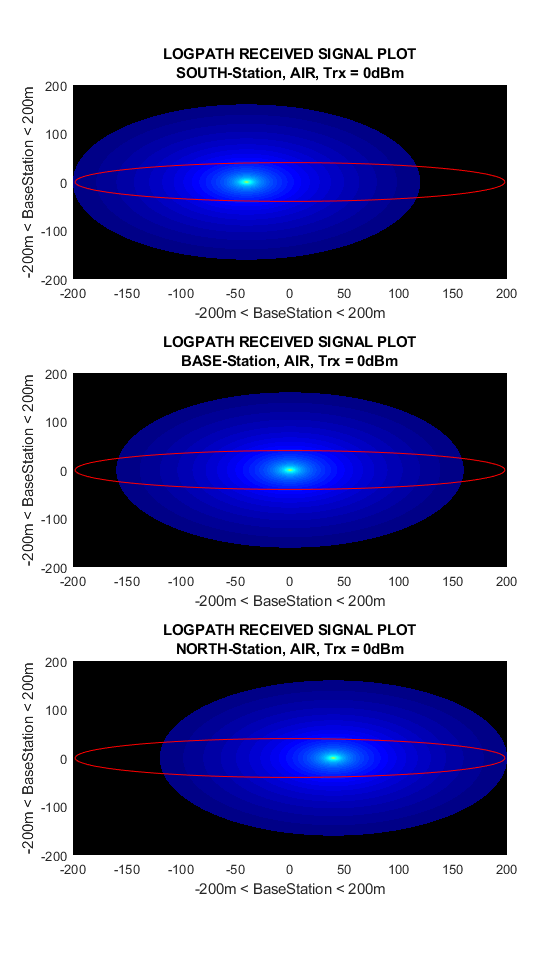
\includegraphics[width=\linewidth]{theory/pathLoss/fig/logpathReceivedSignal_eachStation_air_highSignal.png}
	\caption{Three stations covering the entirety of the racetrack individually.}
	\label{fig:logpathReceivedSignal_eachStation_air_highSignal}
\end{figure}


\begin{figure}[H]
	\centering
	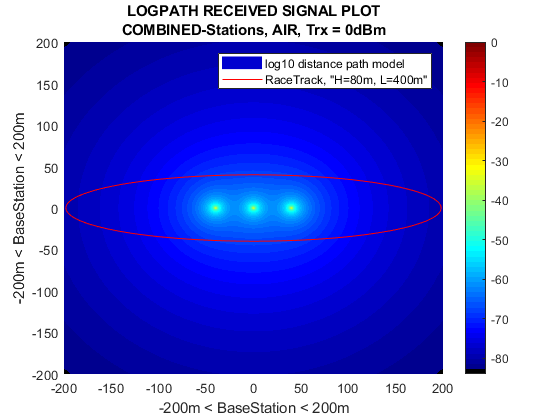
\includegraphics[width=\linewidth]{theory/pathLoss/fig/logpathReceivedSignal_combinedStations_air_highSignal.png}
	\caption{Three stations covering the entirety of the racetrack combined.}
	\label{fig:logpathReceivedSignal_combinedStations_air_highSignal}
\end{figure}

Minimizing the transmission power can lead to extended life time of the individual nodes and the system all together, but at the cost of less coverage area. Figure \ref{fig:logpathReceivedSignal_baseStation_air_lowSignal} shows the single and Figure \ref{fig:logpathReceivedSignal_combinedStations_air_lowSignal} the combined RSSI of the runner node with all nodes using transmission power of $-24dBm$. The size of the race track now is only $7.5\%$ of the full power track. 

%Figure 5
\begin{figure}[H]
	\centering
	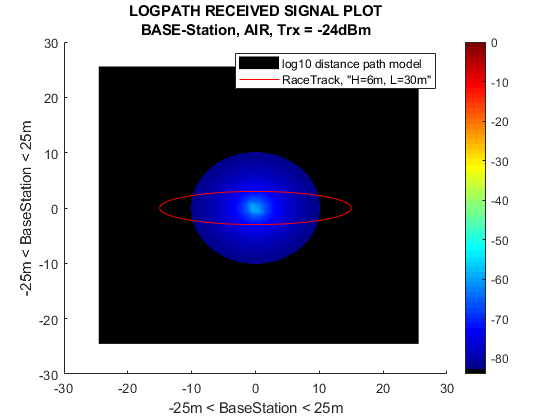
\includegraphics[width=\linewidth]{theory/pathLoss/fig/logpathReceivedSignal_baseStation_air_lowSignal.png}
	\caption{$10.1m$ adequate RSSI for the base station.}
	\label{fig:logpathReceivedSignal_baseStation_air_lowSignal}
\end{figure}

\begin{figure}[H]
	\centering
	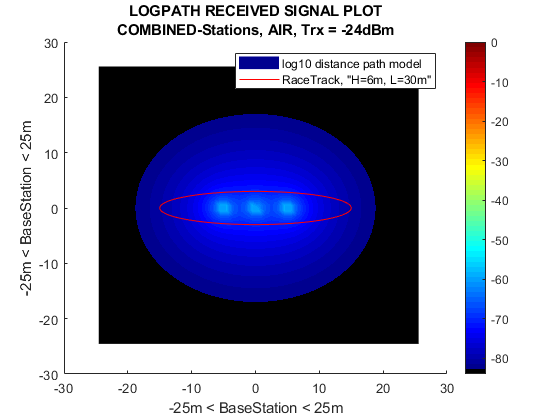
\includegraphics[width=\linewidth]{theory/pathLoss/fig/logpathReceivedSignal_combinedStations_air_lowSignal.png}
	\caption{$10.1m$ Three stations combined RSSI.}
	\label{fig:logpathReceivedSignal_combinedStations_air_lowSignal}
\end{figure}


Further reduction in RSSI can happen for multiple reasons, e.g. reflection, diffraction, scattering and doppler fading. An easy noise model can be to change $\gamma_{air}$ in Equation \ref{eq:rangeEquation} to $\gamma_{building}$, with values taken from page 93 [REF 1]. Figure \ref{fig:logpathReceivedSignal_baseStation_office_lowSignal} and \ref{fig:logpathReceivedSignal_combinedStations_office_lowSignal} shows the distance at minimum Ptr and inside Shannon providing a stunning $0.035\%$ of the coverage related to full power in open AIR.

%Figure 6
\begin{figure}[H]
	\centering
	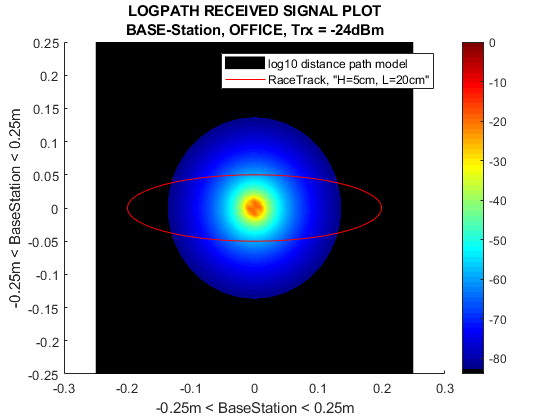
\includegraphics[width=\linewidth]{theory/pathLoss/fig/logpathReceivedSignal_baseStation_office_lowSignal.png}
	\caption{$13.1cm$ adequate RSSI for the base station.}
	\label{fig:logpathReceivedSignal_baseStation_office_lowSignal}
\end{figure}

\begin{figure}[H]
	\centering
	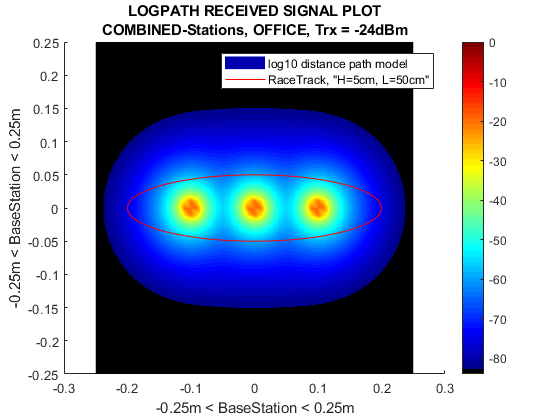
\includegraphics[width=\linewidth]{theory/pathLoss/fig/logpathReceivedSignal_combinedStations_office_lowSignal.png}
	\caption{$13.1cm$ Three stations combined RSSI.}
	\label{fig:logpathReceivedSignal_combinedStations_office_lowSignal}
\end{figure}

\section{Fading}\label{sc:fading}
The above plots all give a good estimate of the RSSI in a stationary clean environment with stationary nodes, but in case of a dynamic environment with obstacles, concepts like fading must be considered. Intrinsic and extrinsic electronic noise set the signal to noise ratio floor of the received signal, but more expensive electronics can compensate for the former noise source, and say no mobile phones at the racetrack can lead to less of the latter noise source, however the RSSI still will experience signal strength drops at times in a dynamic environment. The broadcasting behaviour of the wireless sensor network causes constructive and destructive interference at the receiver, which can lead to deep fading. Deep fading is the scenario in which two or more, out of phase, adequate signals arrive at the receiver simultaneously, leading to a critical destructive interference. The deep fading interferences causes the signal strength to fall below the established noise floor, deeming the signal unreliable or unmeasurable. In the scenario a receiver has experienced a deep fade, depending on the time length, or number of lost packages, the scenario is characterised as a fast fade or a slow fade. This is typically cause by reflection, diffraction or scattering of the signal, causing in line of sight (LOS) signal interfering with a none line of sight (NLOS) signals. The moving of the nodes relative to each other not only has interference, but they have a change in behaviour also. An example of behaviour changing fading is the doppler fading, in which the signal tends to shift in frequency relative to the movement of the sink and the source node. 

\subsection{Doppler Fading}
Following the standard IEEE\_802.15.4, it permits the Telosb to transmit in the ISM  band at frequencies between $2.4$ and $2.4835 GHz$. Having 12 channels, $2 MHz$ wide and separated by $5 MHz$, the TelosB allows a centre frequency signal to shift $\pm 1 MHz$ while still being acknowledged by the receiving channel. Does the signal shift the frequency more than $1 MHz$, the receiving node will simply filter out the signal and the package will be lost. The sign of the shift in frequency depends on the distance between the source and the sink increasing or decreasing. The running node will be changing position relative to the base station at different speeds due to the shape of the track, so an investigation of the effect to the case was made. Firstly, the distance between a package, every quarter of a second, covered by a runner, running at $12kph$, was calculated closest and furthest on the track relative to the base station. The runner is running circular, but the change in distance experienced by the base station will by a straight line leading to doppler frequency found at different speeds relative to track position. The results showed a $29.698Hz$ frequency shift at the end of the track, while the at the top of the track a $26.773Hz$ shift happened. The buffer of $1MHz$ was far beyond the results needed for danger of lost packages due to doppler fading. Just for scalability and flexibility the extreme case was also calculated for the system. Had the runner been running the package distance at approximately $50000kph$ doppler fading would have been an issue. Given the calculated results the project is focusing on fast and slow fading as a simulated instead. See appendix 2 for doppler calculations.

\subsection{Fast Fading and Slow Fading}%TODO Is this how we want appendix (footnote)
Busty bit errors at the receiver is often measured in clusters with different duration or length. Fast fading clusters are typically in the range of tens to hundreds of milliseconds, before the received signal again is adequate, while slow fading clusters are in the range of tens of seconds to minutes. Fast fading and slow fading are both biproducts of the broadcasting behaviour of the nodes, while no clean separation can be made between the two, slow fading is referred to as a shadowing effect and fast fading can be simplified to reflection. E.g. a signal at $2.4GHz$ will have a wavelength of $12.5cm$, given an opposite phased signal every $12.5cm$. If the $2.4GHz$ LOS signal travels $1m$ to the sink and the NLOS signal travels $1.125m$ to the sink, they would cancel each other out. Unfortunately, the calculations of the reflected fading also must consider the directivity of the antenna, since the signal strength also varies at different angles from the source. An antenna with high directivity will since not have a full cancelation at the sink, since the LOS signal will have a higher amplitude than the NLOS signal. The drop-in signal strength can be estimated to be around $30-40dB$ ($60-70dBm$)\footnote{Appendix: 1, page 92}, and this is the values for both slow and fast fading chosen for the simulations in this project. Slow fading can represent diffraction and scattering of the signal from objects in between source and sink, e.g. more runners on the track or the photographer taking images along the route. The slow fading since is modelled as a random stochastic variable with a showing variance visualized through a lognormal fading plot. Given a shadowing variance of $2.22dBm$ and probability of occurrence at $10\%$ for both fast and slow fading, fast fading effect is simulated to last $333 ms$ while slow fading is simulated to last $14s$. Figure \ref{fig:logpathReceivedSignal_baseStation_baseOnly} plots the base station RSSI including fading, while Figure \ref{fig:binaryDeepFading_baseStation_baseOnly} plot the binary, received or lost package, output of the base station. Figure \ref{fig:logpathReceivedSignal_combinedStations_baseOnly} plots the combined stations RSSI including fading, while Figure \ref{fig:binaryDeepFading_combinedStations_baseOnly} plot the binary output of the combined stations and Figure \ref{fig:logpathReceivedSignal_combinedStations_allStations} and \ref{fig:binaryDeepFading_combinedStations_allStations} shows a combined stations plot, but with all three station signals being victims of individual fading patterns. 
\clearpage

%Figure 7, 8 and 9
\begin{figure}[H]
	\centering
	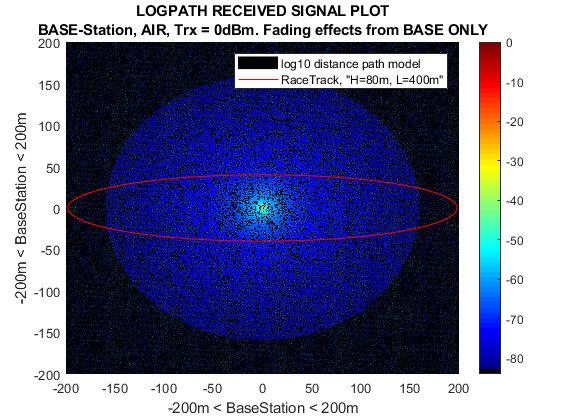
\includegraphics[width=\linewidth]{theory/fading/fig/logpathReceivedSignal_baseStation_baseOnly.png}
	\caption{Base Station RSSI plot after base station experiencing fading}
	\label{fig:logpathReceivedSignal_baseStation_baseOnly}
\end{figure}

\begin{figure}[H]
	\centering
	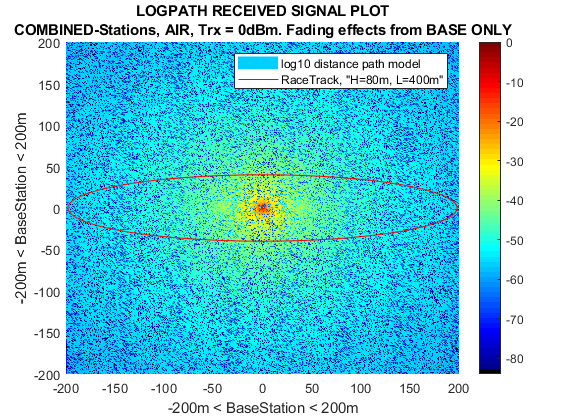
\includegraphics[width=\linewidth]{theory/fading/fig/logpathReceivedSignal_combinedStations_baseOnly.png}
	\caption{Combined Stations RSSI plot after base station experiencing fading}
	\label{fig:logpathReceivedSignal_combinedStations_baseOnly}
\end{figure}

\begin{figure}[H]
\centering
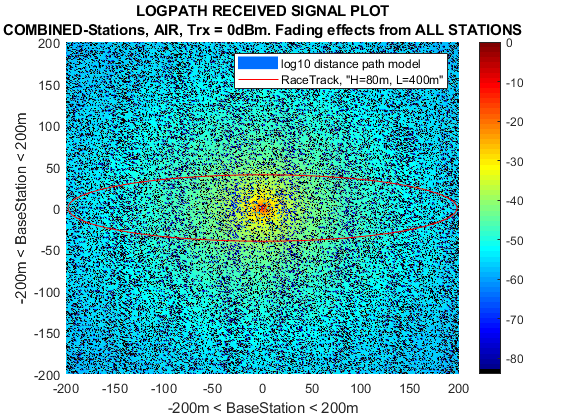
\includegraphics[width=\linewidth]{theory/fading/fig/logpathReceivedSignal_combinedStations_allStations.png}
\caption{Combined Stations RSSI plot after all stations experiencing fading}
\label{fig:logpathReceivedSignal_combinedStations_allStations}
\end{figure}

\begin{figure}[H]
	\centering
	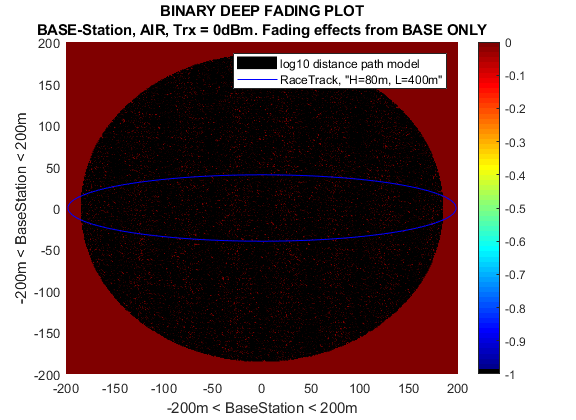
\includegraphics[width=\linewidth]{theory/fading/fig/binaryDeepFading_baseStation_baseOnly.png}
	\caption{Base Station Deep fading plot after base station experiencing fading}
	\label{fig:binaryDeepFading_baseStation_baseOnly}
\end{figure}

\begin{figure}[H]
	\centering
	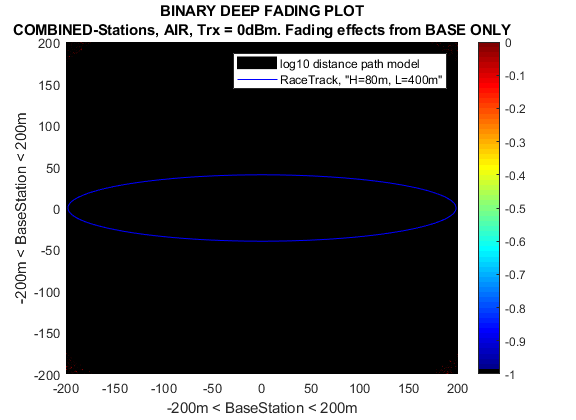
\includegraphics[width=\linewidth]{theory/fading/fig/binaryDeepFading_combinedStations_baseOnly.png}
	\caption{Combined Stations Deep fading plot after base station experiencing fading}
	\label{fig:binaryDeepFading_combinedStations_baseOnly}
\end{figure}

\begin{figure}[H]
	\centering
	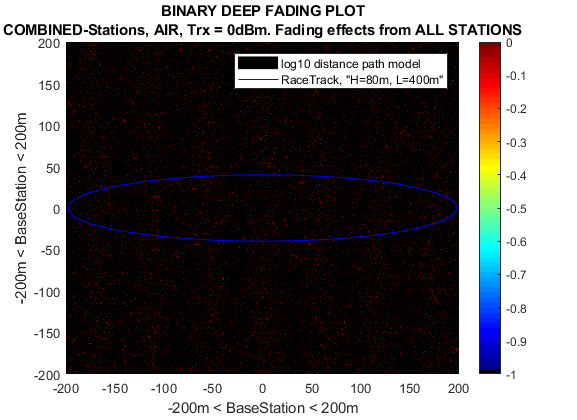
\includegraphics[width=\linewidth]{theory/fading/fig/binaryDeepFading_combinedStations_allStations.png}
	\caption{Combined Stations Deep fading plot after all stations experiencing fading}
	\label{fig:binaryDeepFading_combinedStations_allStations}
\end{figure}



\subsection{Protocol decision example}\label{sc:protocolDecisionExample}
%TODO: Fix figur referencer.
Figure 10 (left) shows the base station's RF input power of a run around the track from start to finish and figure 10 (right) shows it for 47 rounds, which equals a marathon, and each round has different fadings. Figure \ref{fig:recievedSignal_inRange_halfTrack} shows the in-range of the base station packets which needs to be relayed or not.

%Figure 10
%TODO Find matlab document med de to figures i word

%Figure 11
\begin{figure}[h]
	\centering
	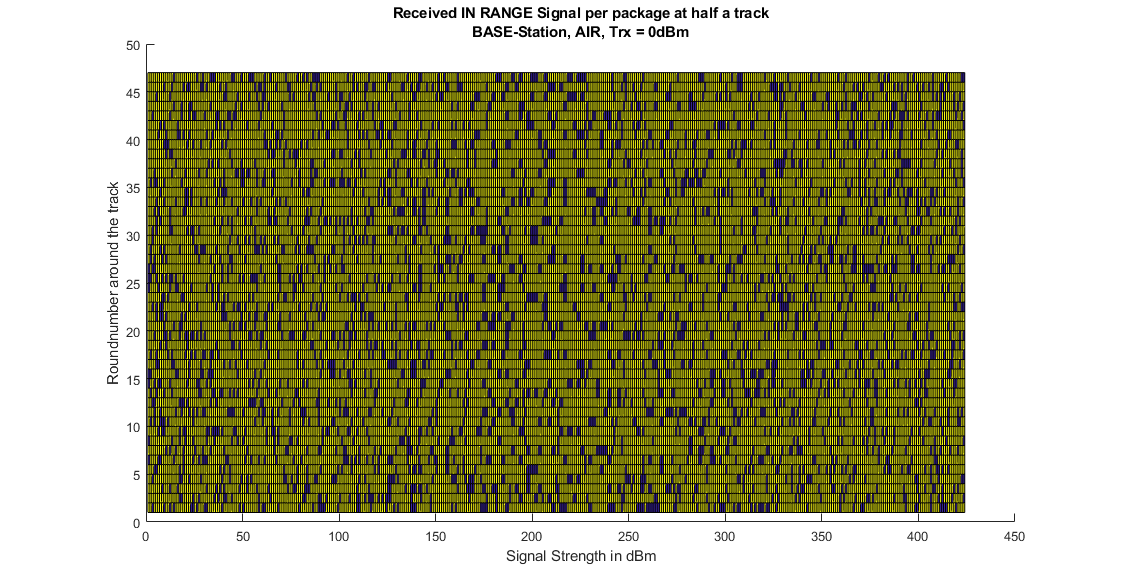
\includegraphics[width=\linewidth]{theory/protocolDecisionExample/fig/recievedSignal_inRange_halfTrack.png}
	\caption{In, half a track, base station RF input power transmitting range ToHopOrNot plot. Blue is relayed packages while yellow is direct package.}
	\label{fig:recievedSignal_inRange_halfTrack}
\end{figure}

\noindent A multi linear regression was fitted on the simulated data with three predictors: Distance, signal strength and whether the packet had been relayed before. The goal was to determine if the node should relay the next packet or not. Since signal strength and distance are strongly correlated in our simulation, due to antenna approximations and the binary behavior of the fading, they cancel each other out, while the previous packet status shows a $10\%$ likelihood of the next packet needing to be relayed. Again, it is expected since the simulations have fading behavior added as a random variable appearing with a $10\%$ likelihood. A real-life trial would be interesting, but is out of scope. Figure \ref{fig:regressionPlot} shows the regression plot with the linear equation added in a legend box.

%Figure 12
\begin{figure}[h]
	\centering
	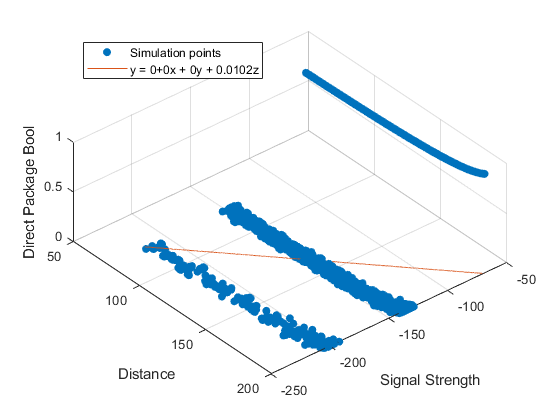
\includegraphics[width=\linewidth]{theory/protocolDecisionExample/fig/regressionPlot.png}
	\caption{Regression plot of the three variables: Distance, signal strength and if previous packet was relayed or not. The regression line is representing a change from direct transmission to relaying.}
	\label{fig:regressionPlot}
\end{figure}

\section{ARQ stop-and-wait method}\label{th:arq}

The ARQ method is a data link-situated telecommunications scheme between two devices. It ensures that information is not lost due to signal fading, infused noise or other network failures and that frames arrive in a correct order. Multiple types of ARQ includes stop-and-wait, go-back-n and selective-repeat. In this project we will be using stop-and-wait because we only transfer a single packet (a heart rate measurement) from the runner and not a large file, i.e. an image. We will now look at the fundamentals of the method. We assume a network that consists of two nodes, $n_1$ and $n_2$, with $n_1$ sending some sort of data to $n_2$: \newline \\
1. $n_1$ wants to send frames with data $d_i$ to $n_2$. It prepares the first frame $d_0$ and transmits it to $n_2$. As soon as its done sending, $n_1$ starts a timer and expects to get an acknowledge frame (ACK) back from $n_2$ within that time telling $n_1$ that the frame has been correctly received. \newline \\
2. $n_2$ receives the frame and sends a ACK frame back to $n_1$. Now $n_1$ can prepare the next frame $d_0+1$. \newline \\
3. In case $n_2$ fail to acknowledge the frame in time, perhaps due to a network glitch or a faulty frame at the receiving end, the timer at $n_1$ will simply run out and it will retransmit frame $d_0$. \newline \\
\noindent Aside from the ARQ stop-and-wait, we add a redundancy check number or parity bit (0 or 1) to all frames. The receiving node uses this number to verify the integrity of the frame, and does only send back an ACK if the frame passes this test. This adds a level of error-correctness to the ARQ method and helps avoid passing malformed data frames around. Two possible pitfalls exist with this version of ARQ: If the transmission medium has a long latency, the sender's timer could run out before the frame reached the receiver, and if the ACK sent by the receiver is damaged, the whole frame would have to be retransmitted. In both cases the receiver gets the same frame twice. One could use the parity bit to recognize duplicate frames, hence solve these problems. In terms of throughput, stop-and-wait falls by the wayside to go-back-N and selective-repeat because each frame has to be acknowledged separately, but may prove more useful in a noisy environment.


\section{Energy Calculations}\label{sc:energyCalculations}
%TODO add section reference for energy lab
In every wireless network system energy consumption is a must to evaluate. Based on measurement, see section ???, some calculations were made. Since power consumption is not the main investigation of the project, only lifetime for the base station is done in theory. An assumption of every package is send directly to the sink successfully and immediately a respond is send also successfully. Total latency between the two nodes is set as constant to 12 milliseconds and an overshoot time at powerup from sleep mode is also constant at 50 milliseconds and $40\%$ extra energy related to receiving energy. Overshoot after wakeup is modelled as a gaussian function as shown in Figure \ref{fig:gaussianDistributionsOfVoltagePeak} for max energy wakeup. Table 1 shows the lifetime of the base station at six different scenarios all assuming two full AA-batteries.
Scenario 1: Full power at transmission and otherwise always listening for packages.
Scenario 2: Min power at transmission and otherwise always listening for packages.
Scenario 3: Full power at transmission, only listening for packages when receiving and no overshoot.
Scenario 4: Min power at transmission, only listening for packages when receiving and no overshoot.
Scenario 5: Full power at transmission, only listening for packages when receiving and overshoot at power up.
Scenario 6: Min power at transmission, only listening for packages when receiving and overshoot at power up.
Calculations are in appendix ?? and even though it cost to power up from sleep mode, it is still gives longer life time to put the nodes to sleep.

%Figure 13
\begin{figure}[H]
	\centering
	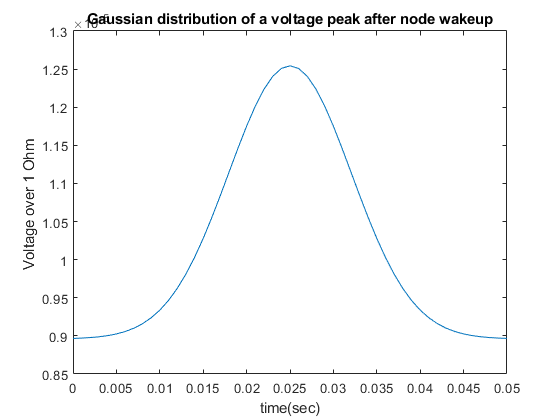
\includegraphics[width=\linewidth]{theory/energyCalculations/fig/gaussianDistributionsOfVoltagePeak.png}
	\caption{Start up voltage peak after sleep mode.}
	\label{fig:gaussianDistributionsOfVoltagePeak}
\end{figure}

\section{Implementation}\label{ch:implementation}

This chapter describes how the theory discussed in chapter \ref{ch:theory} has been implemented in our solution. We have divided the chapter into a overall section about the ARQ protocol and then sections per node, that is base station, the relay nodes and the runner node. For better readability, code snippets of the actual implementation has been turned into pseudo code. To view the nesC code please see the appendix.

\noindent The chapter end with the section Energy Lab. In this section energy consumption will be discussed at different send/receive scenarios.

\subsection{Generic ARQ implementation}\label{sc:overall}

The ARQ stop-and-wait method has been implemented on all nodes in the system. Figure \ref{fig:tohopornotarqsequence} is a sequence diagram of the  protocol implementation and shows how data requests are initiated by the base station and forwarded either directly to the runner (left side) or via a relay station (right side). Adding to this is the parity bit calculations to verify the integrity of received frames. This is conduced when a frame is received in either base station or one of the other nodes.

\begin{figure}[h]
	\centering
	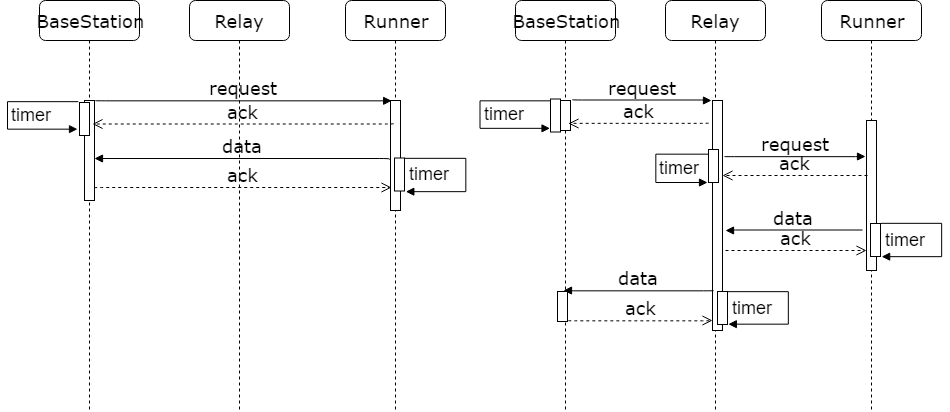
\includegraphics[width=1\linewidth]{implementation/overall/toHopOrNotArqSequence}
	\caption{The flow of data and acknowledgment messages between the nodes.}
	\label{fig:tohopornotarqsequence}
\end{figure}

\noindent The basics of the communications between the nodes are as follows: \\ \newline
1. The base station requests data at a certain time interval defined by a timer. When the timer runs out, it decides whether is should send the request directly or via one of the relays by using our protocol. To the request is attached a counter ($n = 0, 1, 2, 3$ -> $n$) and a sequence number (0 or 1) used by the receiver to verify the frame. When the radio is ready to transmit, it is forwarded to a specific node and the ARQ timer starts. It it now the responsibility of the receiving node to carry on the request. The receiver will send back a ACK frame to the base station if validation succeeded.\\ \newline
2. If the request reached the runner first, it will use the attached counter to calculate a new parity bit and compare this to the one in the request. If they match, it sends back an ACK followed by a data message containing the current heart rate of the athlete. A counter and a sequence number is attached to this as well.\\ \newline
3. The base station receives the data message, checks the parity bit, and saves it. It has now successfully obtained the heart rate.\\ \newline
4. If the base station decide to relay the request, the same procedure applies for the relay nodes. It is now the job of the relay to acknowledge the request, communicate with the runner using ARQ, obtain the data and send it back to the base station.\\ \newline
\noindent With ARQ and parity bit checking we archive a simple but reliable data-link connection between nodes and a way to discard damaged frames. One particular area of concern was the configuration of the timers, as they have to be consistent throughout the network. Obviously when relaying, the base station must take into account the turnaround time and possible retransmissions of the relay and the runner node before sending a new one. The base station timer ($Ba_t$) must be larger than the relay's ($Re_t$) and the runner's ($Ru_t$) combined, so $Ba_t$ > $Re_t$ + $Ru_t$ for the protocol to work correctly.

\section{Base station}\label{sc:basestation}

The base station is the master node in our setup. It is responsible for three import tasks: Initiating data requests, decide if the runner is out of range and keep track of past events. Figure \ref{fig:tohopornotarqsequence} shows the overall flow of data, but we shall examine the more detailed parts here.

\noindent The main control loop is started by a timer every $s$ second. It asserts if the runner is deemed out of range by calling a function and uses the feedback (either true or false) to increase an error counter that is used to change destination node. In other words, when a certain number of errors have occurred on the current link, we change request destination (from directly to relaying or vice versa). Listing \ref{lst:basestation1} is an example.
\noindent
\begin{minipage}[t]{0.95\linewidth}
	\begin{lstlisting}[language=Python, numbers=none, caption=XXX, label={lst:basestation1}]
Timer0.fired() {
	if out of range and link is direct {
		if the error count is below max
			use_next_destination
		else
			increase_error_count
	}
	if link is direct
		send_a_message_direct
	if link is relay to node north
		send_a_message_to_north
	if link is relay to node south
		send_a-message_to_south
}
	\end{lstlisting}
\end{minipage}

\noindent Next is how the base station determines if the runner is out range. When new replies are received directly from the runner (it starts in range) we save the RSSI\footnote{RSSI is a scalar register value on the CC2420 radio calculated from the RF input power in dBm.} value in a FIFO(First In First Out) queue with a length of 10. In such a queue, new data is inserted at back and taken out from the front. This means that the latest RSSI value of the runner is the back entry, with $n=0,1,2 ... 8$ being previous positions. Our algorithm takes a mean of these and multiplies it with a weighted score. If the latest position is lower than the mean, it is added to the weighted mean of the previous positions. If it is greater the average is then subtracted from it. The result constitutes a new estimated position of the runner. Listing \ref{lst:basestation2} is an example.

\noindent
\begin{minipage}[t]{0.95\linewidth}
\begin{lstlisting}[language=Python, numbers=none, caption=XXX, label={lst:basestation2}]
bool isOutOfRange {
	if current size of queue is not max
		return
	for(i = 0; i < queue_size; i++)
		previousPos += queue_part[i]
		
	lastPos = queue_back_entry
	mean = previousPos/queue_size
	
	if lastPos is less than mean
		newPos = (lastPos*1)+(mean*0.1);
	else
		newPos = (lastPos*1)-(mean*0.1);
	
	if(newPos is larger than threshold)
		return true;
	return false;
}
\end{lstlisting}
\end{minipage}

\noindent The weights used can be changed to put more empathize on the previous positions or more on the latest. Resulting on it acting more or less fast on new network conditions newest received packet.

\subsection{Relay}\label{sc:relay}
The Relay nodes in this setup are slaves to the base station. Their functionality is to relay messages to the Runner node, where the base station node is out of reach. Because of this the Relay node listens to the network and in case of being spoken to, will reply with an acknowledge and further send data to the Runner node. In case that the Relay node is not able to get in contact with the Runner node after three times, it sends an error message to the Base station.

\begin{minipage}[t]{0.95\linewidth}
	\begin{lstlisting}[caption=Receive message event of Relay., label={lst:relay1}]
event message_t * Receive.receive(message_t *msg, void *payload, uint8_t len){
	if (len == sizeof(requestMessage)) {
		requestMessage* reqmsg = (requestMessage*) payload;
		
		if (reqmsg->relayNodeid == TOS_NODE_ID) {
			// Send Acknowledge
			sendAcknowledge(reqmsg);
			
			if (reqmsg->data == 0) {	
				requestFromBase = *reqmsg;
				call Timer0.startPeriodic(TIMER0_PERIOD_MILLI);		
			}
			else {
				requestFromRunner = *reqmsg;
				call Timer1.startPeriodic(TIMER1_PERIOD_MILLI);
			}
		}
	}
	\end{lstlisting}
\end{minipage}

\noindent On listing \ref{lst:relay1} the main functionality of the Relay nodes can be seen. The Relay nodes are always in need of commands to them before sending a command themselves, they won't work on their own and therefore relies on requests from the Base station and answers from the Runner.

\subsection{Runner}\label{sc:runner}

The runner node's task in our WSN is to respond to data request messages sent from the base station or the relay nodes, as seen in the sequence digram in figure \ref{fig:tohopornotarqsequence}. The node contains various settings that can configured as constants, so they are easy to change eg. the transmit channel and the radiation power of the antenna. When it receives a packet it will check that the packet was intended for the runner and if so it will send an ACK to the requester and get ready to send the data as a subsequent reply.

\begin{minipage}[t]{0.95\linewidth}
\begin{lstlisting}[label={lst:runner1}, caption={Runner receives requests and responds.}]
Receive.receive(Message pkt){
	if pkt is requestMessage {
		if request is for runner {
			send_Acknowledgement
			Timer_sendDataTorequester
		}
	} 
}
\end{lstlisting}
\end{minipage}

\noindent The data contains the heart rate of the runner and in this scenario we just return a constant value. When sending data to the requesting node, it will start a timer and if it does not receive an ACK within a fixed time, it will resend the message three times followed by giving up on that reply.

\begin{minipage}[t]{0.95\linewidth}
\begin{lstlisting}[label={lst:runner2}, caption={Runner sends data packet with runner's heart rate.}]
sendData() {
	if If is not AntenaBusy {
		responsePacket_pulseData add runner_heart_beat
		if AMSend_send(responsepkt) is SUCCESS {
			AntenaBusy to TRUE
			resendCounter++
		}
	}
	if resendCounter is bigger then and equal to TRIES_TO_RESEND {
		resendCounter = 0
	}
}
\end{lstlisting}
\end{minipage}

\section{Energy Lab}\label{sc:energylab}

To test the 
\section{Test and performance}\label{ch:testAndPerformance}

This section describes the test configuration and how we measured the performance of our protocol.

\begin{figure}[h]
	\centering
	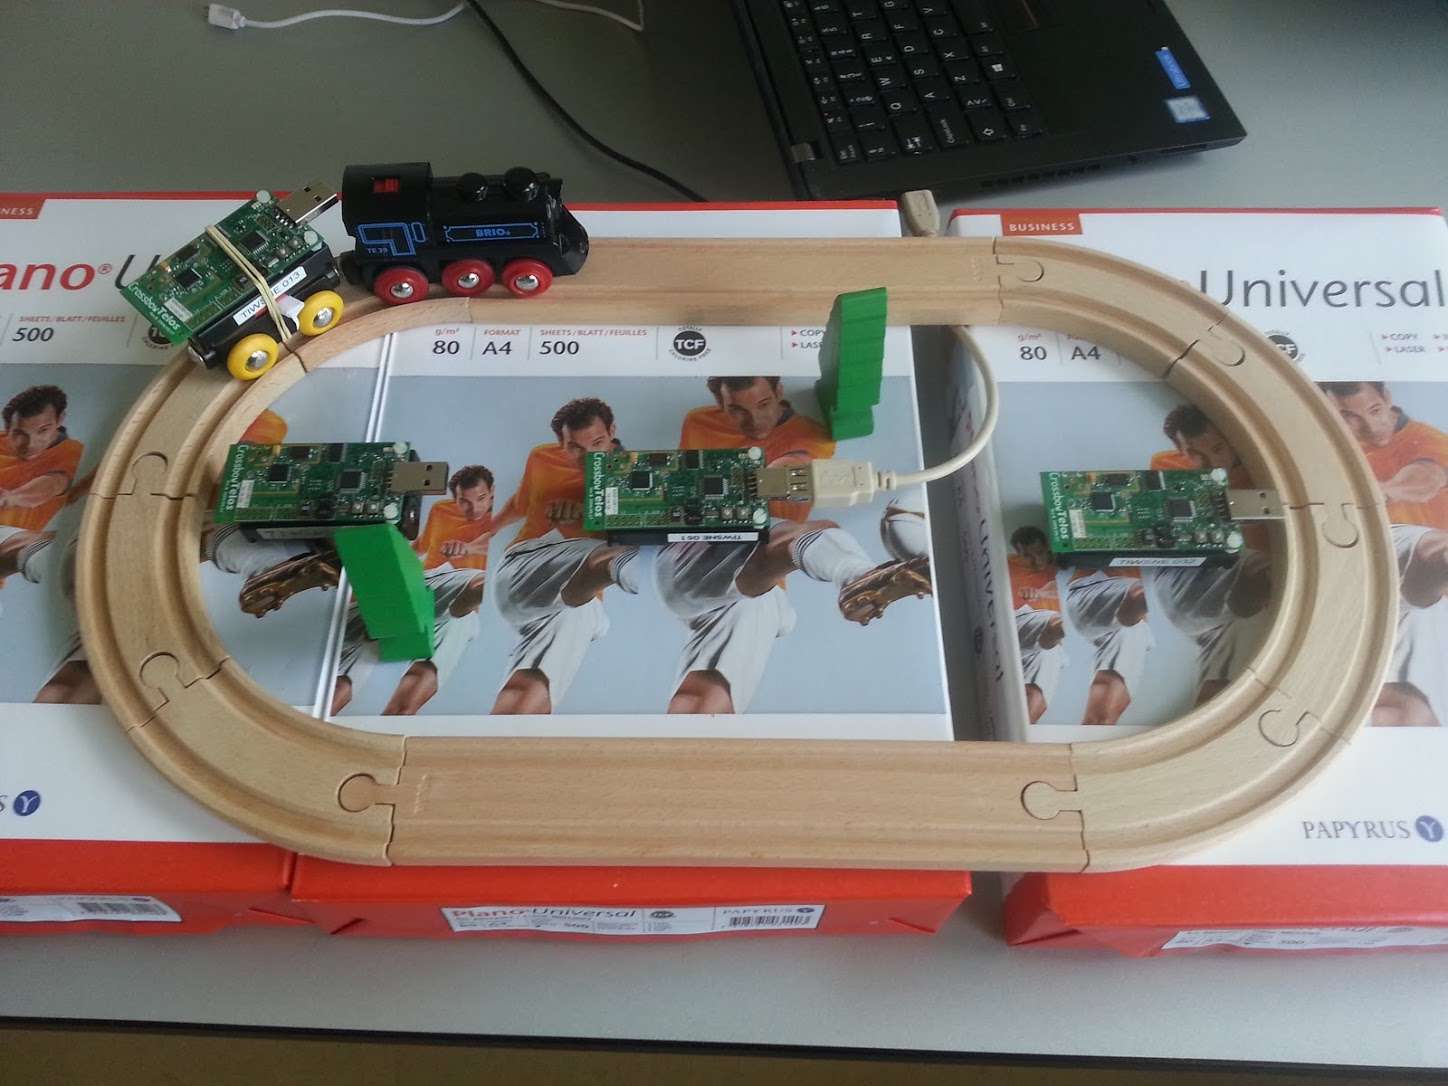
\includegraphics[width=1\linewidth]{testAndPerformance/setup/setup}
	\caption{A Brio toy train track with the base, north and south relay stations in the center and the runner put on top of the train.}
	\label{fig:testSetup}
\end{figure}

\section{Setup}\label{sc:setup}
To test our original scenario described in the Introduction on page \pageref{ch:introduction} we built a smaller version of the running track. To get a constant speed and a track to run tests on we use a Brio\texttrademark train to symbolism a human runner that runs a track. The speed of the runner was set to $12\dfrac{km}{hr}$ but the Brio train had a speed of $0.2604\dfrac{km}{hr}$. The track we used in the theory part was 906.17m long and the runner would run a marathon which is 46.56km and therefor is 46.56 rounds. Using the standard Brio track pack we build a track with length of 43.5cm. In the theory we send $4\dfrac{packets}{sec}$ and that means our time per packet should be $\dfrac{1}{4sec} = 0.250ms$ and therefor about $ 1.087*10^3$ packets per round. But our as our train is slowing than the runner and the track was shorter we needed to account for the differences between our test setup and the theory made in section \ref{table:datascenarios} on page \pageref{table:scenarios}. Our inital calulations showed that we needed to send XXX packets and that was not possible use to limits of the hardware, as seen in Figure POWERFIFG REF it takes 15ms to send a packet and that is not accounting for other things the TelosB might be during so as handling computations. Therefor we divided the packets per round by 4 $ \dfrac{packetsPerRound}{4} = 271.852 $ and therefor needing $57.016 ms$ per packet



\begin{figure}[H]
	\centering
	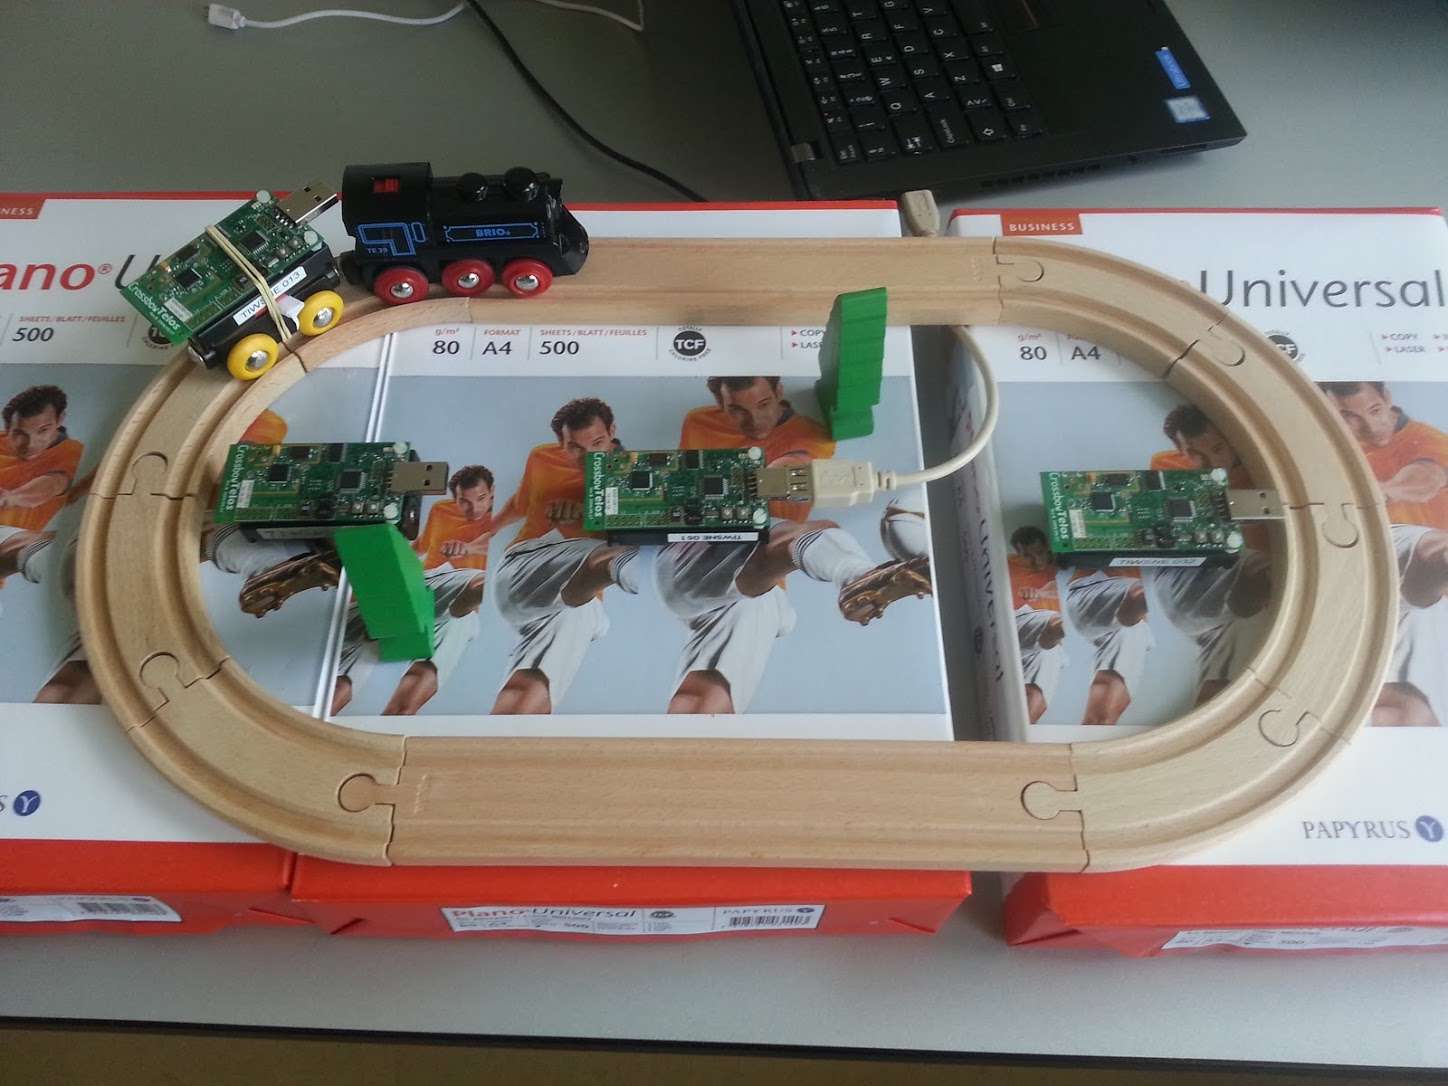
\includegraphics[width=1\linewidth]{testAndPerformance/setup/setup}
	\caption{The train track withbasestation, north and south relay nodes and the runner. }
	\label{fig:testSetup}
\end{figure}



\section{WiFi conditions}\label{sc:wifi}
In our test we used two different WiFi chanenls (4 and 11) and we found the best and the worst by using the WiFi Analyzer app from the Android app store\cite{Farproc@gmail.com2018}. As seen in figure \ref{fig:wifionthetestday}, channel 11 is used by Aarhus University WiFi but channel 4 looks rather free, so we picked these two as seen in table \ref{table:scenarios}.

\begin{figure}[h]
	\centering
	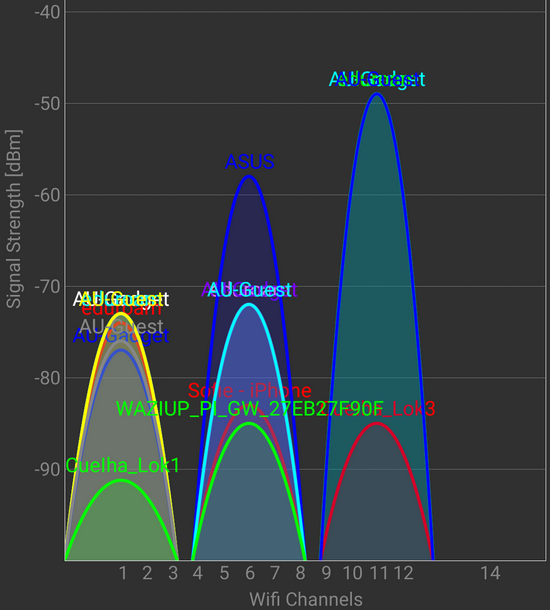
\includegraphics[width=0.6\linewidth]{testAndPerformance/wifi/wifiOnTheTestDay}
	\caption{WiFI on the test day. Channel 11 was busy and Channel 4 was a quiet channel}
	\label{fig:wifionthetestday}
\end{figure}

We ran 4 tests for 48 minutes each testing our protocol with different channels and track lengths.

\begin{table}[h]
	\centering
	\begin{tabular}{|l|l|l|l|l|l|l|} \hline
		Scenario & \pbox{18cm}{Channel} & \pbox{18cm}{RSSI} & \pbox{18cm}{Length of track} \\ \hline
		1 & 11 & -40 & 43.5cm \\ \hline
		2 & 11 & -40 & 56cm \\ \hline
		3 & 4 & -40 & 43.5cm \\ \hline
		4 & 4 & -40 & 56cm \\ \hline
	\end{tabular}
	\caption{Test scenarios performed.}
	\label{table:scenarios}
\end{table}					
\section{Results}\label{ch:results}

Using the test setup and mechanics described in section \ref{ch:testAndPerformance}, we conducted a experiment of four different scenarios. We wanted to see whether the hopping frequency would increase, when we increased the circumference of the track, evaluate the packet sent/loss ratio and measure the overall perception of data. The test results would indicate if our relaying algorithm, the implemented stop-and-wait ARQ protocol and distance measurements were correct and working. All results are gathered from the base station and can be found in appendix 10. To quickly iterate the parameters measured in the test runs: \\

\noindent \textbf{\textit{n} request packets sent ($p_1$):} Number of packets sent from the base station over the course of the test. These include retries due to ARQ timers expiring. Read this number as "times we have asked for data".

\noindent \textbf{\textit{n} packets relayed to node 1 ($p_2$):} Number of packets relayed to north relay station.

\noindent \textbf{\textit{n} packets relayed to node 2 ($p_3$):} Number of packets relayed to south relay station.

\noindent \textbf{\textit{n} ACK's received ($p_4$):} Number of acknowledgments received by the ARQ protocol. The closer this number is to the packets sent, the more stable the data link connection between our endpoints is.

\noindent \textbf{\textit{n} DATA's received ($p_5$):} Number of data packets received. Ideally, this should be close to the packets sent as well. If $p_5$<$p_1$, then $p_1$-$p_5$ request packets were not replied.

\noindent \textbf{\textit{n} packets not acknowledged in time ($p_6$):} Number of packets not acknowledged before the ARQ timer ran out. This is strongly related to the timers on the base station and heavily influenced by interference and signal noise. Also in our test set-up we tried to get as much data from the runner as possible, so timers were strict.\\

\noindent Table \ref{table:datascenarios1} and \ref{table:datascenarios2} show the final result of each completed scenario lasting 48 minutes each, which equals about $168$ (small track) and $130$ (large track) rounds with the train. Both tracks have the same amount of total packages sent, $12280$. Each minute we recorded parameters $p_1$ to $p_6$. All are initially set to zero. We decided not to change the RSSI threshold in each scenario.

\begin{table}[h]
	\centering
	\begin{tabular}{|c|c|c|c|c|} \hline
		Sn. & \pbox{10cm}{$p_1$} & \pbox{17cm}{$p_2$} & \pbox{17cm}{$p_3$} & \pbox{17cm}{$p_2 + p_3$} \\ \hline
		1 & 29148 & 4066 & 3512 & 7578 \\ \hline
		2 & 29838 & 8115 & 8499 & 16614 \\ \hline
		3 & 29258 & 3706 & 4021 & 7727 \\ \hline
		4 & 30523 & 1232 & 8425 & 9657 \\ \hline
	\end{tabular}
	\caption{Data from scenarios 1-4 for parameters 1-3.}
	\label{table:datascenarios1}
\end{table}

\begin{table}[h]
	\centering
	\begin{tabular}{|c|c|c|c|} \hline
		Sn. & \pbox{17cm}{$p_4$} & \pbox{17cm}{$p_5$} & \pbox{17cm}{$p_6$} \\ \hline
		1 & 22169 & 34167 & 20700 \\ \hline
		2 & 17880 & 23563 & 21111 \\ \hline
		3 & 21944 & 32830 & 21244 \\ \hline
		4 & 19137 & 28874 & 23188 \\ \hline
	\end{tabular}
	\caption{Data from scenarios 1-4 for parameters 4-6.}
	\label{table:datascenarios2}
\end{table}

\noindent As expected, the results vary depending on the track length and the channel used. When using a length of $56cm$ (scenario 2 and 4), we see $p_5 \leq p_1$, meaning the base station received the same or less data packets than requested. In scenario four they are even fairly close. If $p_5 > p_1$, it could be due to fading or missed timers. Also worth noting is the increased use of relays ($p_2$ and $p_3$) when the length is $56cm$. Changing channels between 11 and 4 seem to lower the difference between $p_1$ and $p_5$ as well.

\noindent Figure \ref{fig:noackreceived} shows the correlation between the number of ACK's received, $p_4$, at the base station per packet sent from it. These numbers should be close to each other. Scenario 2 received a large number of ACK's around the 24408 packet sent mark, perhaps due to deep fading.

\begin{figure}[h]
	\centering
	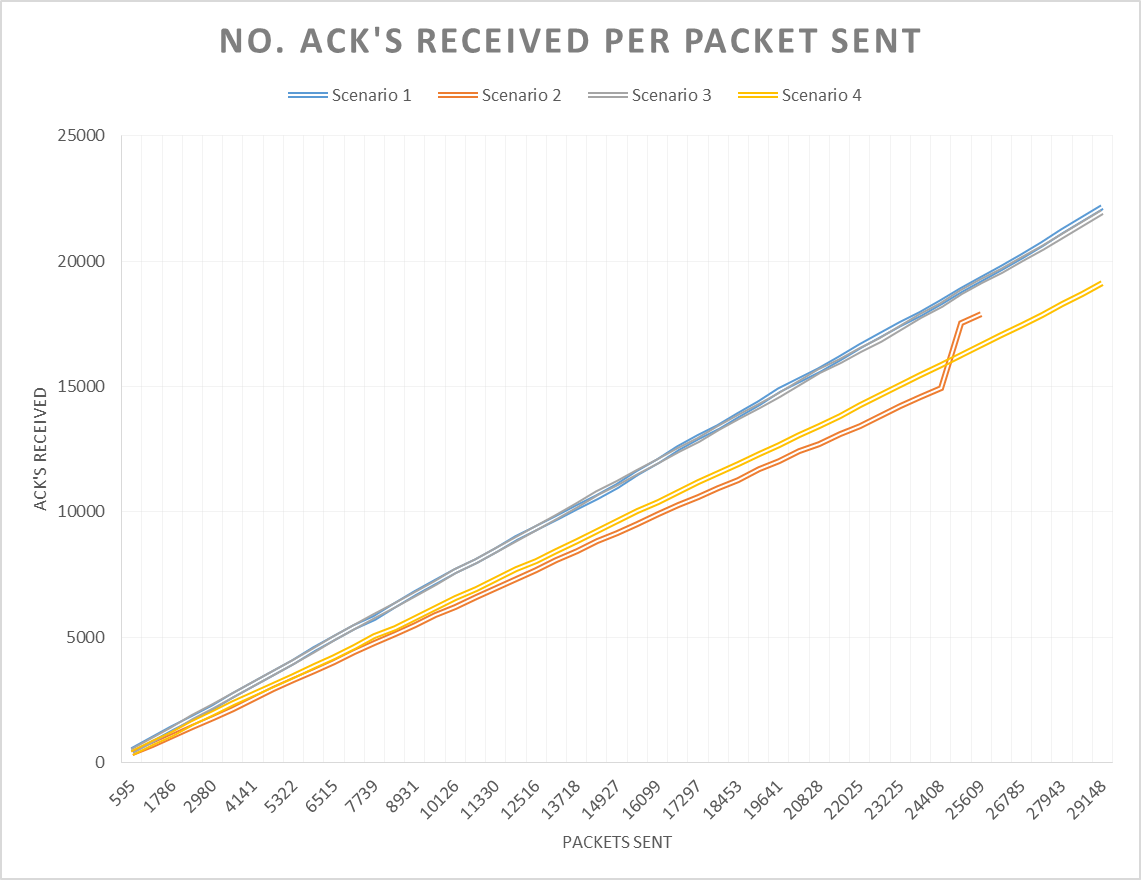
\includegraphics[width=1\linewidth]{results/NoAckReceived}
	\caption{No. ACK's received per packet sent.}
	\label{fig:noackreceived}
\end{figure}

\noindent Figure \ref{fig:nodatareceived} shows the number of data packets received, $p_5$, from the runner node either direct or via one of the relays per packet sent. Scenario 1 and 3 ($length = 43.5cm$) follows each other slightly, however changing channel from 11 to 4 decrease the amount of additional packets received ($p_5 > p_1$) when using $length = 43.5cm$. Scenario 4 looks to be the most successful one, as the number of data packets received is close to the number of requests sent. We reflect on this at the end of results. Scenario 1 and 3 sees more data packets being received than requested. A probable cause is a packet not being acknowledged in time by the base station, so the runner will resend it, even though it might already have been received by the base station.

\begin{figure}[h]
	\centering
	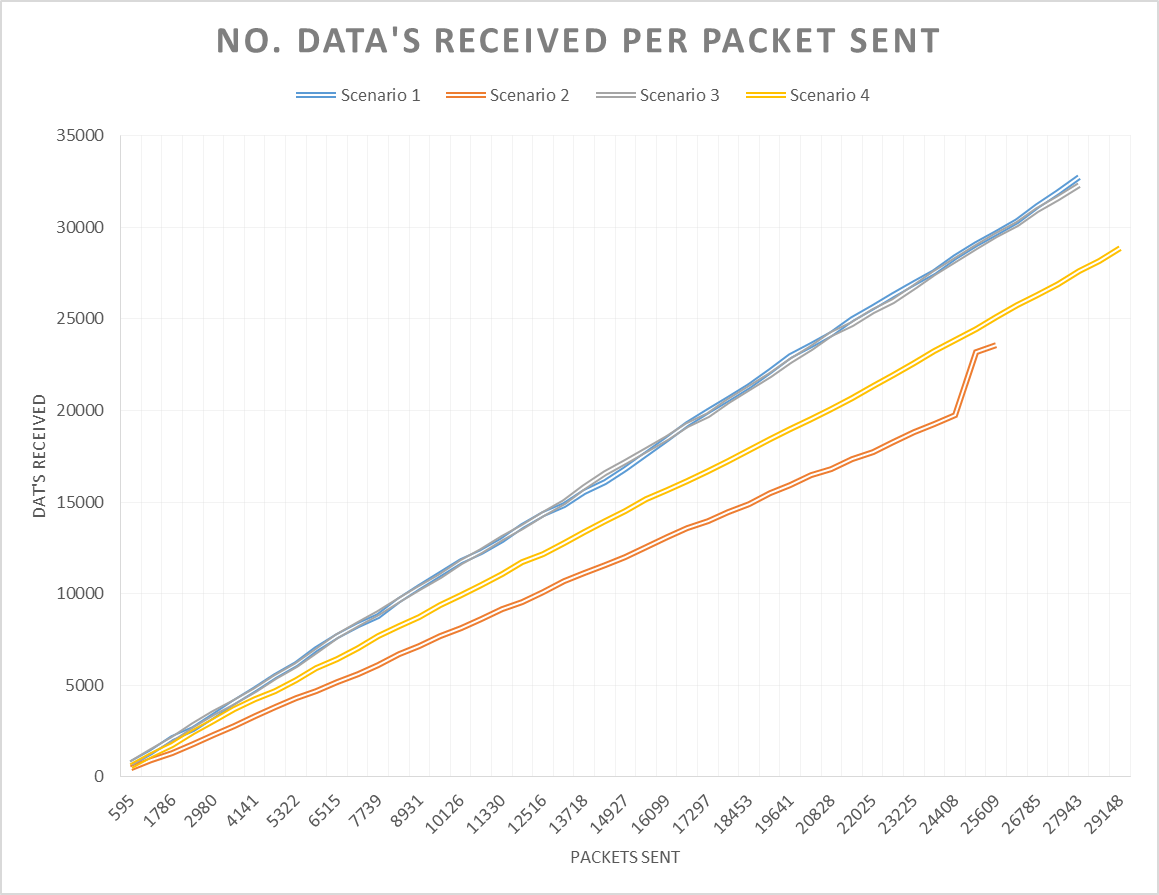
\includegraphics[width=1\linewidth]{results/NoDataReceived}
	\caption{No. DATA's received per packet sent.}
	\label{fig:nodatareceived}
\end{figure}

\noindent Figure \ref{fig:nopacketsrelayed} shows the number of data relayed to the north  and south relay station combined per packet sent. As expected, scenario 2 and 4 ($length=56cm$) relays more packets, now that the runner node will be out of reach from the base station for a longer period of time. It might even be that neither can reach the runner due to deep fading. Calculations made in Appendix 1 show the minimum theoretical packets send from the base station, which must be relayed at each of the track length. The total packets sent from the base station ideally is 12280, the minimum relayed packets send from the the base station for scenario 1 and 3 are 2355 packets, and for scenario 2 and 4 are 4961 packets. Both the number of relayed packets and the total number of packets send from the base station is flawed compared to theory and this will be further discussed in the discussion, but the inter scenario relative test results follow the theory well. The base station should send a request to the runner after a specified time to investigate if the runner has returned into direct communication reach, of the base station. Alternative the RSSI of the relaying node could be evaluated by the base station to give an idea of the runner node position.

\begin{figure}[h]
	\centering
	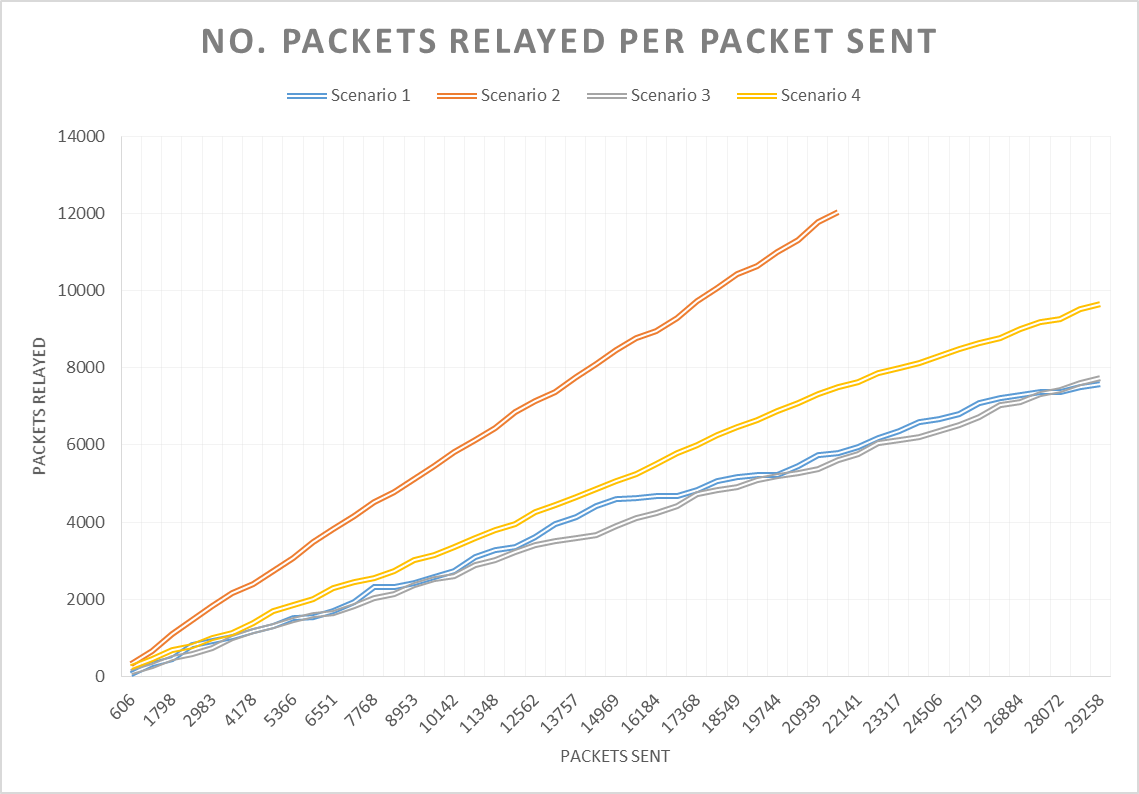
\includegraphics[width=1\linewidth]{results/NoPacketsRelayed}
	\caption{No. packets relayed per packet sent.}
	\label{fig:nopacketsrelayed}
\end{figure}

\noindent Figure \ref{fig:nopacketsnotackintime} shows the number of packets not acknowledged in time per packet sent. All scenarios follows each-other, which points to a systematically error either due to strict timers or fading issues. An error that channel or length does not seem to affect. We noticed during the live testing that more ARQ errors occurred when communicating directly rather than relaying. Figure \ref{fig:nopacketsrelayedscenario2} and \ref{fig:nopacketsrelayedscenario4} show how the two scenarios that relay the most packets (2 and 4) distribute the data among our two relay stations (north and south) per packet relayed. A bit strange is the sudden drop of packets relayed to the north station in scenario 4, figure  \ref{fig:nopacketsrelayedscenario4}. Probable reason is fading.

\begin{figure}[H]
	\centering
	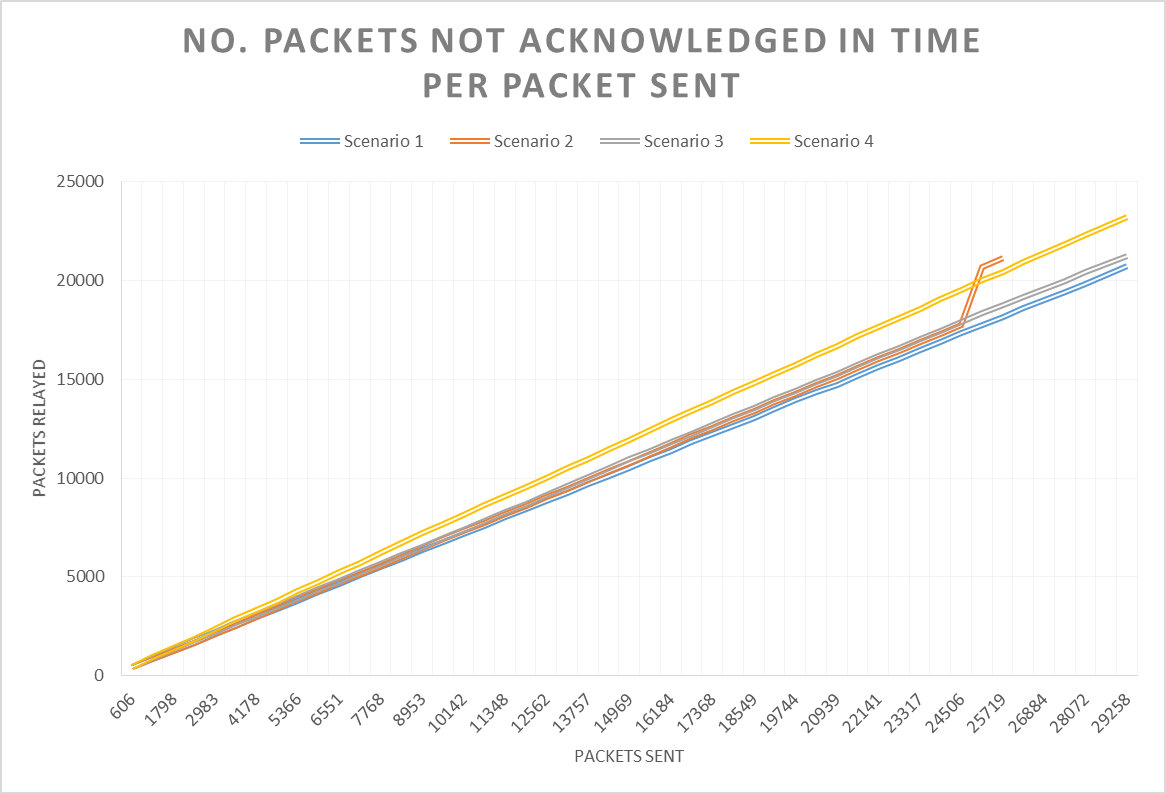
\includegraphics[width=1\linewidth]{results/NoPacketsNotACKInTime}
	\caption{No. packets not acknowledged in time.}
	\label{fig:nopacketsnotackintime}
\end{figure}

\begin{figure}[H]
	\centering
	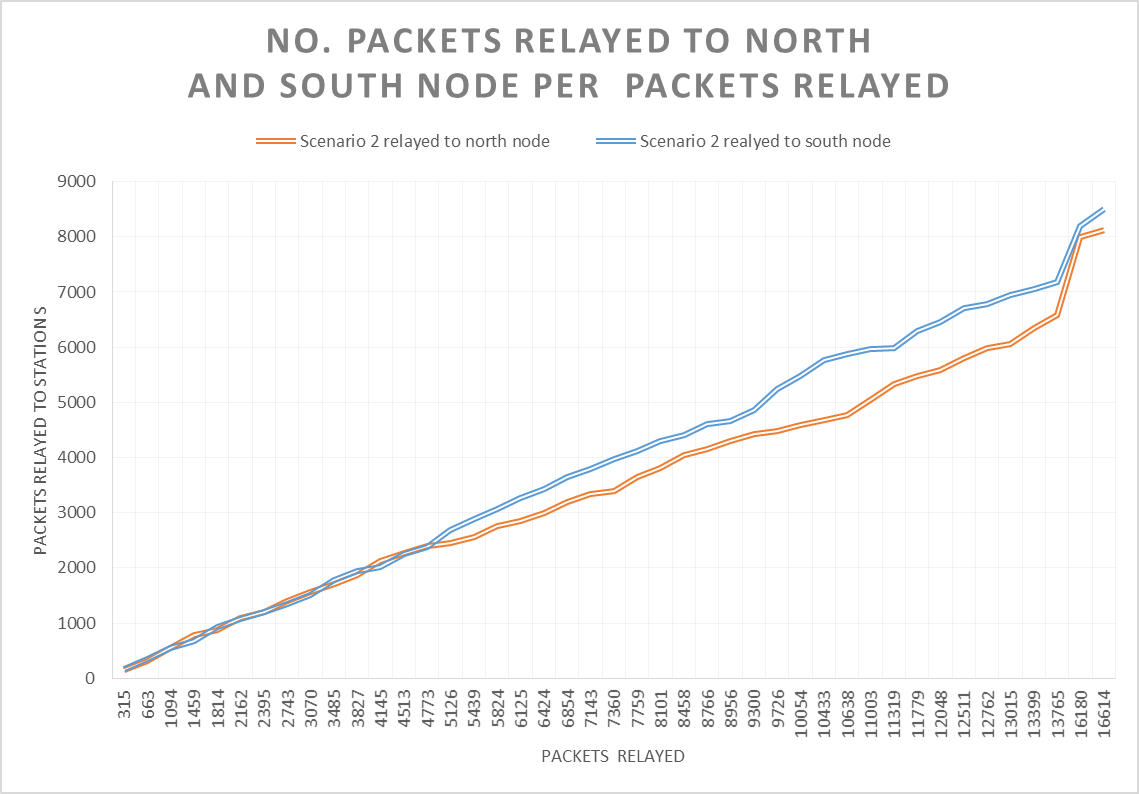
\includegraphics[width=1\linewidth]{results/NoPacketsRelayedScenario2}
	\caption{No. packets relayed to north and south node in scenario 2.}
	\label{fig:nopacketsrelayedscenario2}
\end{figure}

\begin{figure}[H]
	\centering
	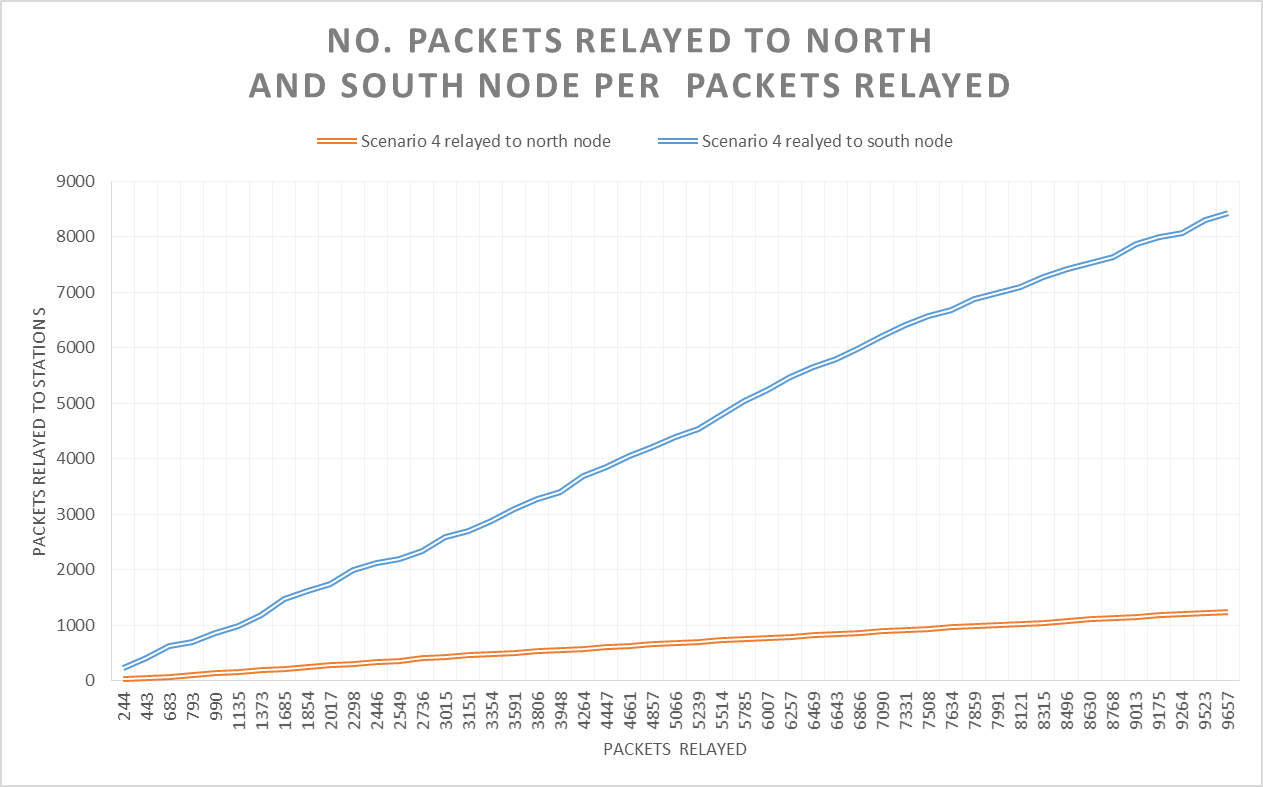
\includegraphics[width=1\linewidth]{results/NoPacketsRelayedScenario4}
	\caption{No. packets relayed to north and south node in scenario 4.}
	\label{fig:nopacketsrelayedscenario4}
\end{figure}

\noindent In terms of event quality (number of packets requested ($p_1$) vs. received ($p_5$)) the different scenarios has various characteristics. A optimal scenario is one where the number of requests sent is close to the number of data packets received, that is $p_1 \approx p_5$. If $p_1 > p_5$, we have asked for more events than received, i.e. packets have not been send or lost. If $p_1 < p_5$, we have received more events than asked for, i.e. information overload. Table \ref{table:eventquality} shows event quality for each scenario (1-4). Surprisingly scenario 4 provides the overall best event quality, and not scenario 3, i.e. using a channel with less traffic and increasing the length of the track, hence relying more on the relay stations.

\begin{table}[h]
	\centering
	\begin{tabular}{|c|l|l|r|} \hline
		Sn. & \pbox{4cm}{Requests \\ sent} & \pbox{18cm}{DATA's \\ received} & \pbox{18cm}{\% Quality \\ difference.} \\ \hline
		1 & 29148 & 34167 & $17.2\%$ \\ \hline
		2 & 29838 & 23563 & $-21.0\%$ \\ \hline
		3 & 29258 & 32830 & $12.2\%$ \\ \hline
		4 & 30523 & 28874 & $-5.4\%$ \\ \hline
	\end{tabular}
	\caption{Event quality from scenarios 1-4.}
	\label{table:eventquality}
\end{table}

\noindent Looking at the energy consumption, the smaller the track the less total energy will be consumed because of less messages relayed. This result in less total energy consumed because the relays are inactive, assuming the relays are sleeping when inactive. However this is not true in the test scenarios, but in a optimized scenario this would be the case and is therefore concluded upon. Energy consumption per packet sent can be found in table \ref{table:energyConsumption}. As shown, the total energy consumption of the system as well as that of the base station itself is higher in scenario 2 and 4 because of the extra request messages send through relays. The conclusion is that the more messages or packets that needs relaying the more energy is consumed overall. Surprisingly again scenario 3 was not the optimal setup, but it turned out to be scenario 1.

\begin{table}[H]
	\centering
	\begin{tabularx}{\linewidth}{|c|X|X|}
		\hline
		Sn.	& Total energy [Ah]	& Base station percentage used [\%]	\\ \hline
		1			& $0.577$			& $8.81$							\\ \hline
		2			& $0.731$			& $9.02$							\\ \hline
		3			& $0.581$			& $8.84$							\\ \hline
		4			& $0.632$			& $9.23$							\\ \hline
	\end{tabularx}
	\caption{Energy consumption assuming a specific cost per packet sent. "Total energy" is the energy consumed by the whole system. "Base station percentage used" is the percentage of the total energy used by the base station.}
	\label{table:energyConsumption}
\end{table}

\noindent The result of both event quality and energy consumption show that the size of the track matters. Increasing the size of the track and adding more relays improves the event quality but also increases the energy consumption. It all come down to a trade-off between event quality and energy consumption. Track size results show that the effect on event quality overshadow the drawback of intensified energy consumption when increasing the track size.											
\chapter{Discussion}

There are a few things that could have been done to improve various parameters in this project. Some could be entire projects in their own. To improve battery life of the relays stations and the runner, one could implement a medium access (MAC) protocol such as the S-MAC that make nodes periodically sleep and auto-synchronize their sleep schedules. As we have shown, solely using the antenna uses a lot of energy and the S-MAC would help mitigate challenge in a WSN. Because of the way our case works, we have an estimated position of the runner at time $t$, which we can exploit to our advantage. When the runner is at the north area of the track therefore being covered by the north relay station, it makes little sense to have the south relay turned on and consuming energy. A way to optimize this would be to send a message to the relay not in use and make it turn off its antenna and enter sleep mode, then wake it up later when the runner is within range of that station.

%TODO: Why exactly would that make the network more scaleable? Explain :)
\noindent If we made the relay nodes able to relay between each other then that would open of the network to be scale of network. This would make it able to cover a even bigger track. Then we could also make some nodes to enter sleep mode because we would know the runner was on the other side of the track.

\noindent Our protocol in the current state is susceptible to attackers who takes advantage of the fact that our base station will keep using a relay if it can continue to give a good RSSI and heart rate data. This abuse would stop our wireless sensor network from operating correctly.								      
\chapter{Conclusion}		


%----------------------------------------------------------------------------------------
%	REFERENCE LIST
%----------------------------------------------------------------------------------------

\bibliographystyle{plainnat}
\bibliography{bibliography/Mendeley/mendeley} \label{sc:bibliography}

\section*{Appendixes}
\noindent Appendix1

\noindent A pdf-file with various mathcad calculations. Range calculations, Doppler spread and Samples per round.\\

\noindent Appendix2

\noindent A txt-file with various matlab code. PowerCircle, PowerCircleOffice, FadingPlots, ToHopOrNotToHop and Protocol\_Decision.\\

\noindent Appendix3

\noindent A pdf-file with mathcad calculations for the running track and the train track scenario.\\

\noindent Appendix4

\noindent A zip-file with the nesC code for BaseStation.\\

\noindent Appendix5

\noindent A zip-file with the nesC code for Relay.\\

\noindent Appendix6

\noindent A zip-file with the nesC code for Runner.\\

\noindent Appendix7

\noindent A zip-file with the different results from various energy laboratory tests.\\

\noindent Appendix8

\noindent A zip-file with the different nesC codes for various energy laboratory tests.\\

\noindent Appendix9

\noindent A pdf-file with matlab code for lifetime calculations.\\

\noindent Appendix10

\noindent An excel-file with results from train track scenario.\\			

%----------------------------------------------------------------------------------------

\end{document}
